\section{Limits on associated heavy Higgs-boson production}

Using the 1-lepton search, 95\% CL upper limits on the associated heavy Higgs boson production cross sections times branching ratios are derived for the three signal processes studied: $b\bar{b}H$, $t\bar{t}H$, and $tbH^{+}$. 
The upper limits on $b\bar{b}H$\ and $t\bar{t}H$\ production can be applied to $b\bar{b}A$ and $t\bar{t}A$ production respectively, since there are no significant differences in the kinematic distributions at the reconstructed level. The limits are derived under the assumption that only a single signal process at a time contributes in the signal regions, which makes these limits conservative. Stronger limits would be obtained if simultaneous contributions from four mass-degenerate states ($H$, $A$, and $H^\pm$) had been considered.

Figure \ref{sec:vlq:fig:hbsm1} shows the observed and expected upper limits on $\sigma(pp \to b\bar{b}H) \times {\rm BR}(H \to t\bar{t})$
as a function of the heavy Higgs-boson mass $m_H$, compared to benchmark theoretical predictions within a Type-I and
Type-II 2HDM.  In both cases, the obtained limits are more than one order of magnitude above the largest predictions in the
alignment limit ($\cos(\beta-\alpha)=0$), which correspond to  $\tan\beta$ values of about 0.1 and 5 respectively. The limited sensitivity 
of this search is due to the small signal acceptance, since often at least one of the associated $b$-quarks is not reconstructed and/or $b$-tagged.

\begin{figure}[t!]
\begin{subfigure}{0.5\textwidth}
  \centering
  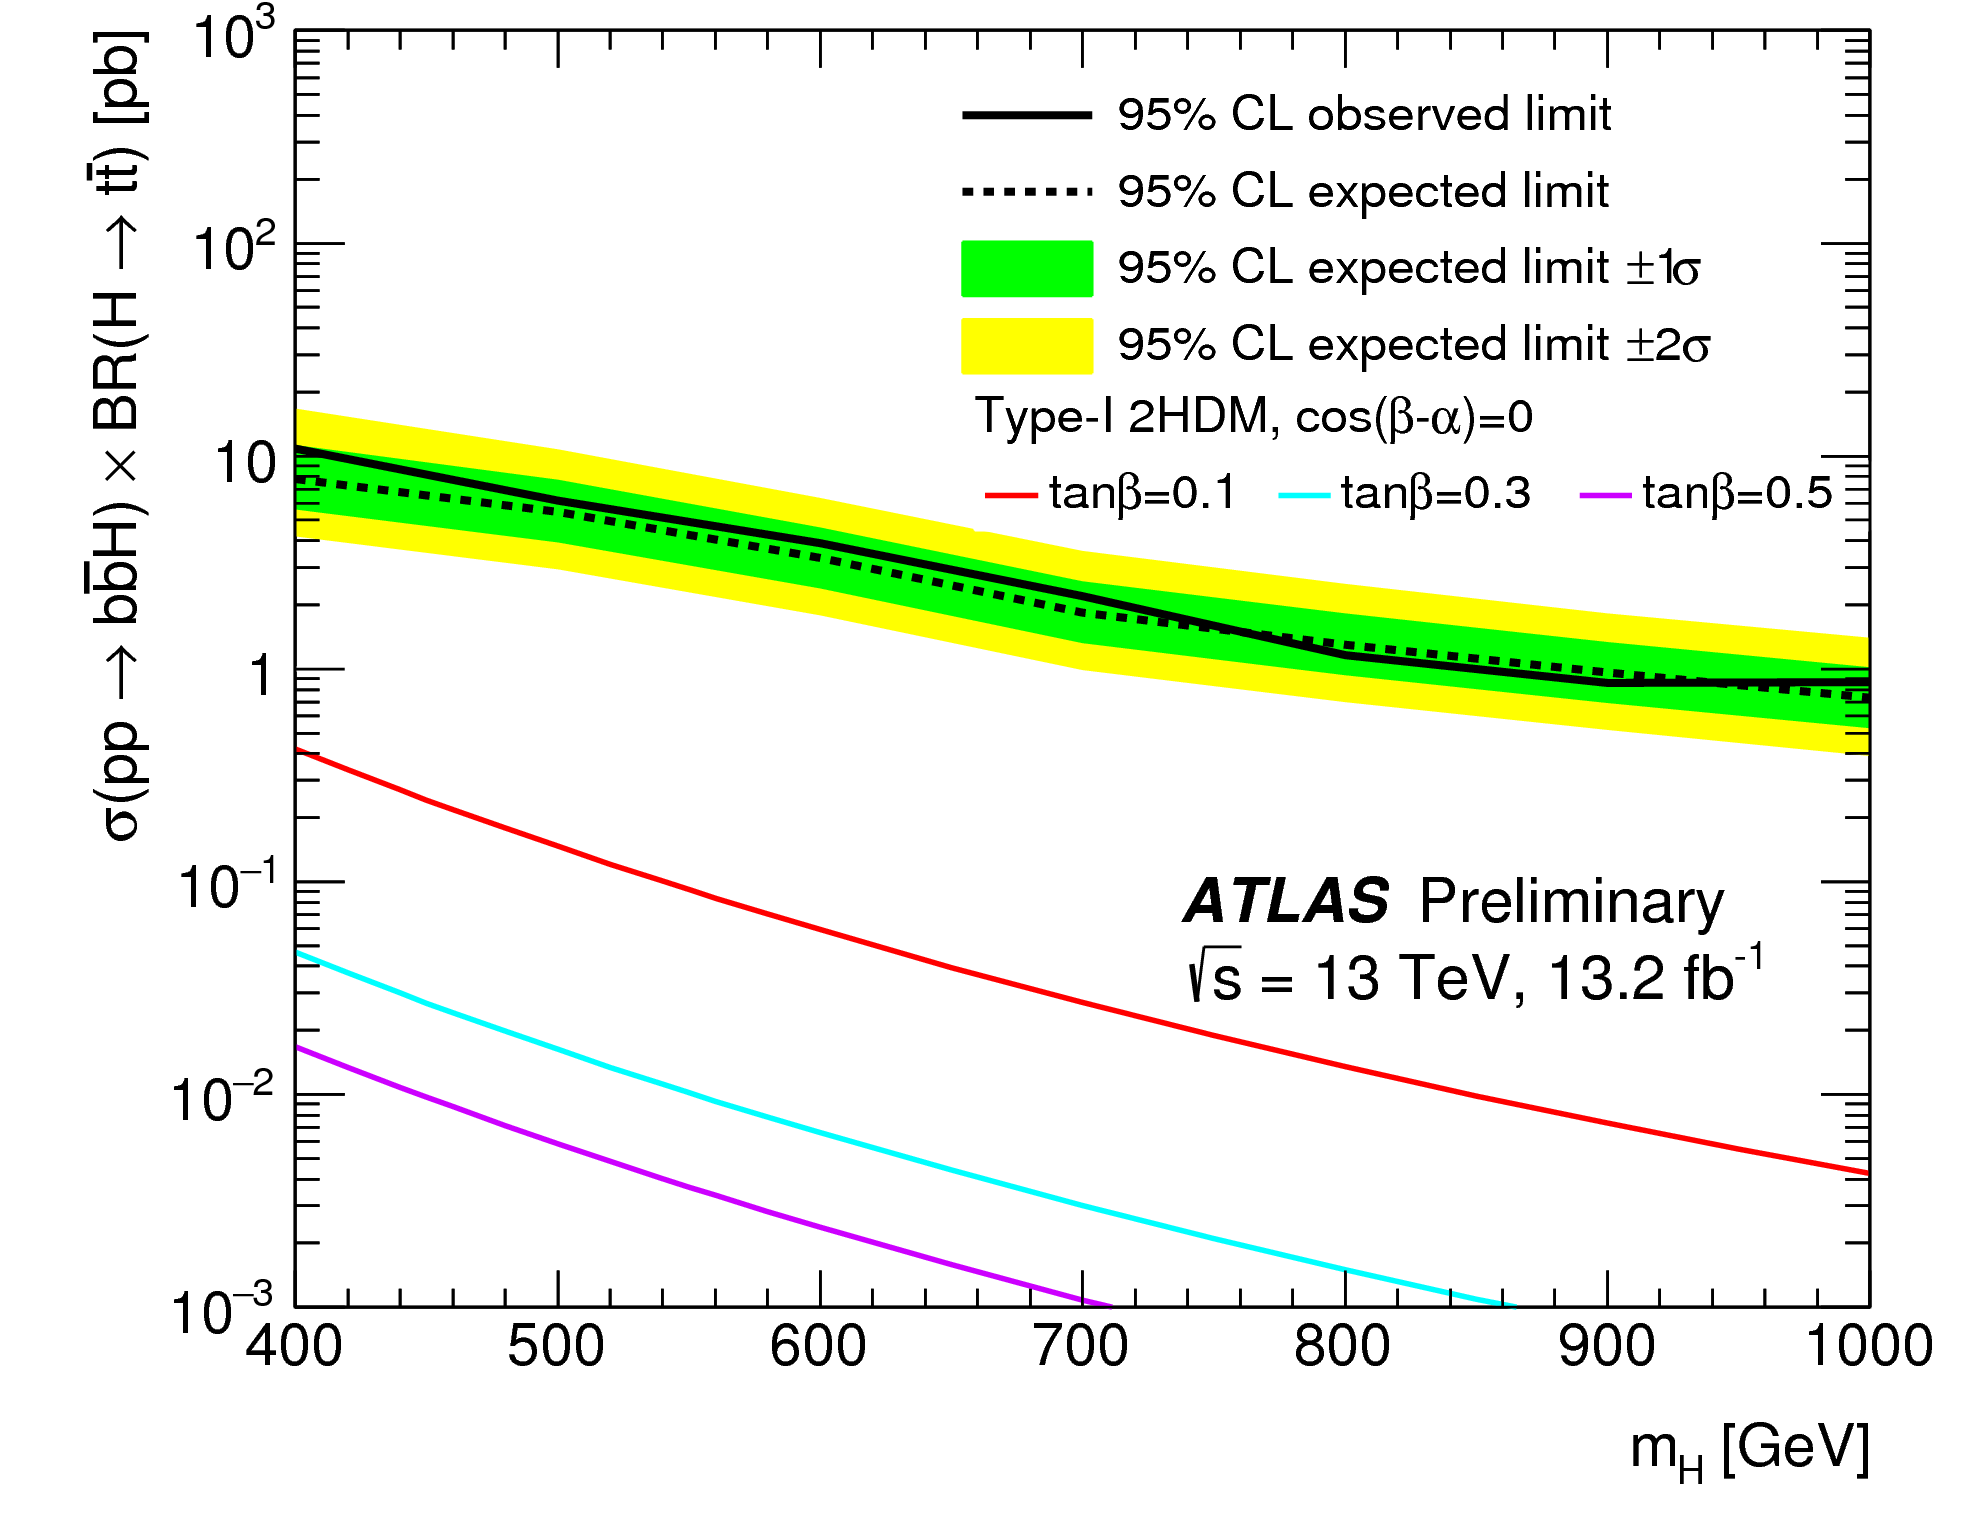
\includegraphics[width=0.9\textwidth]{figures/VLQ/fig_21a.png}
  \caption{}
  \label{}
\end{subfigure}
\begin{subfigure}{0.5\textwidth}
  \centering
  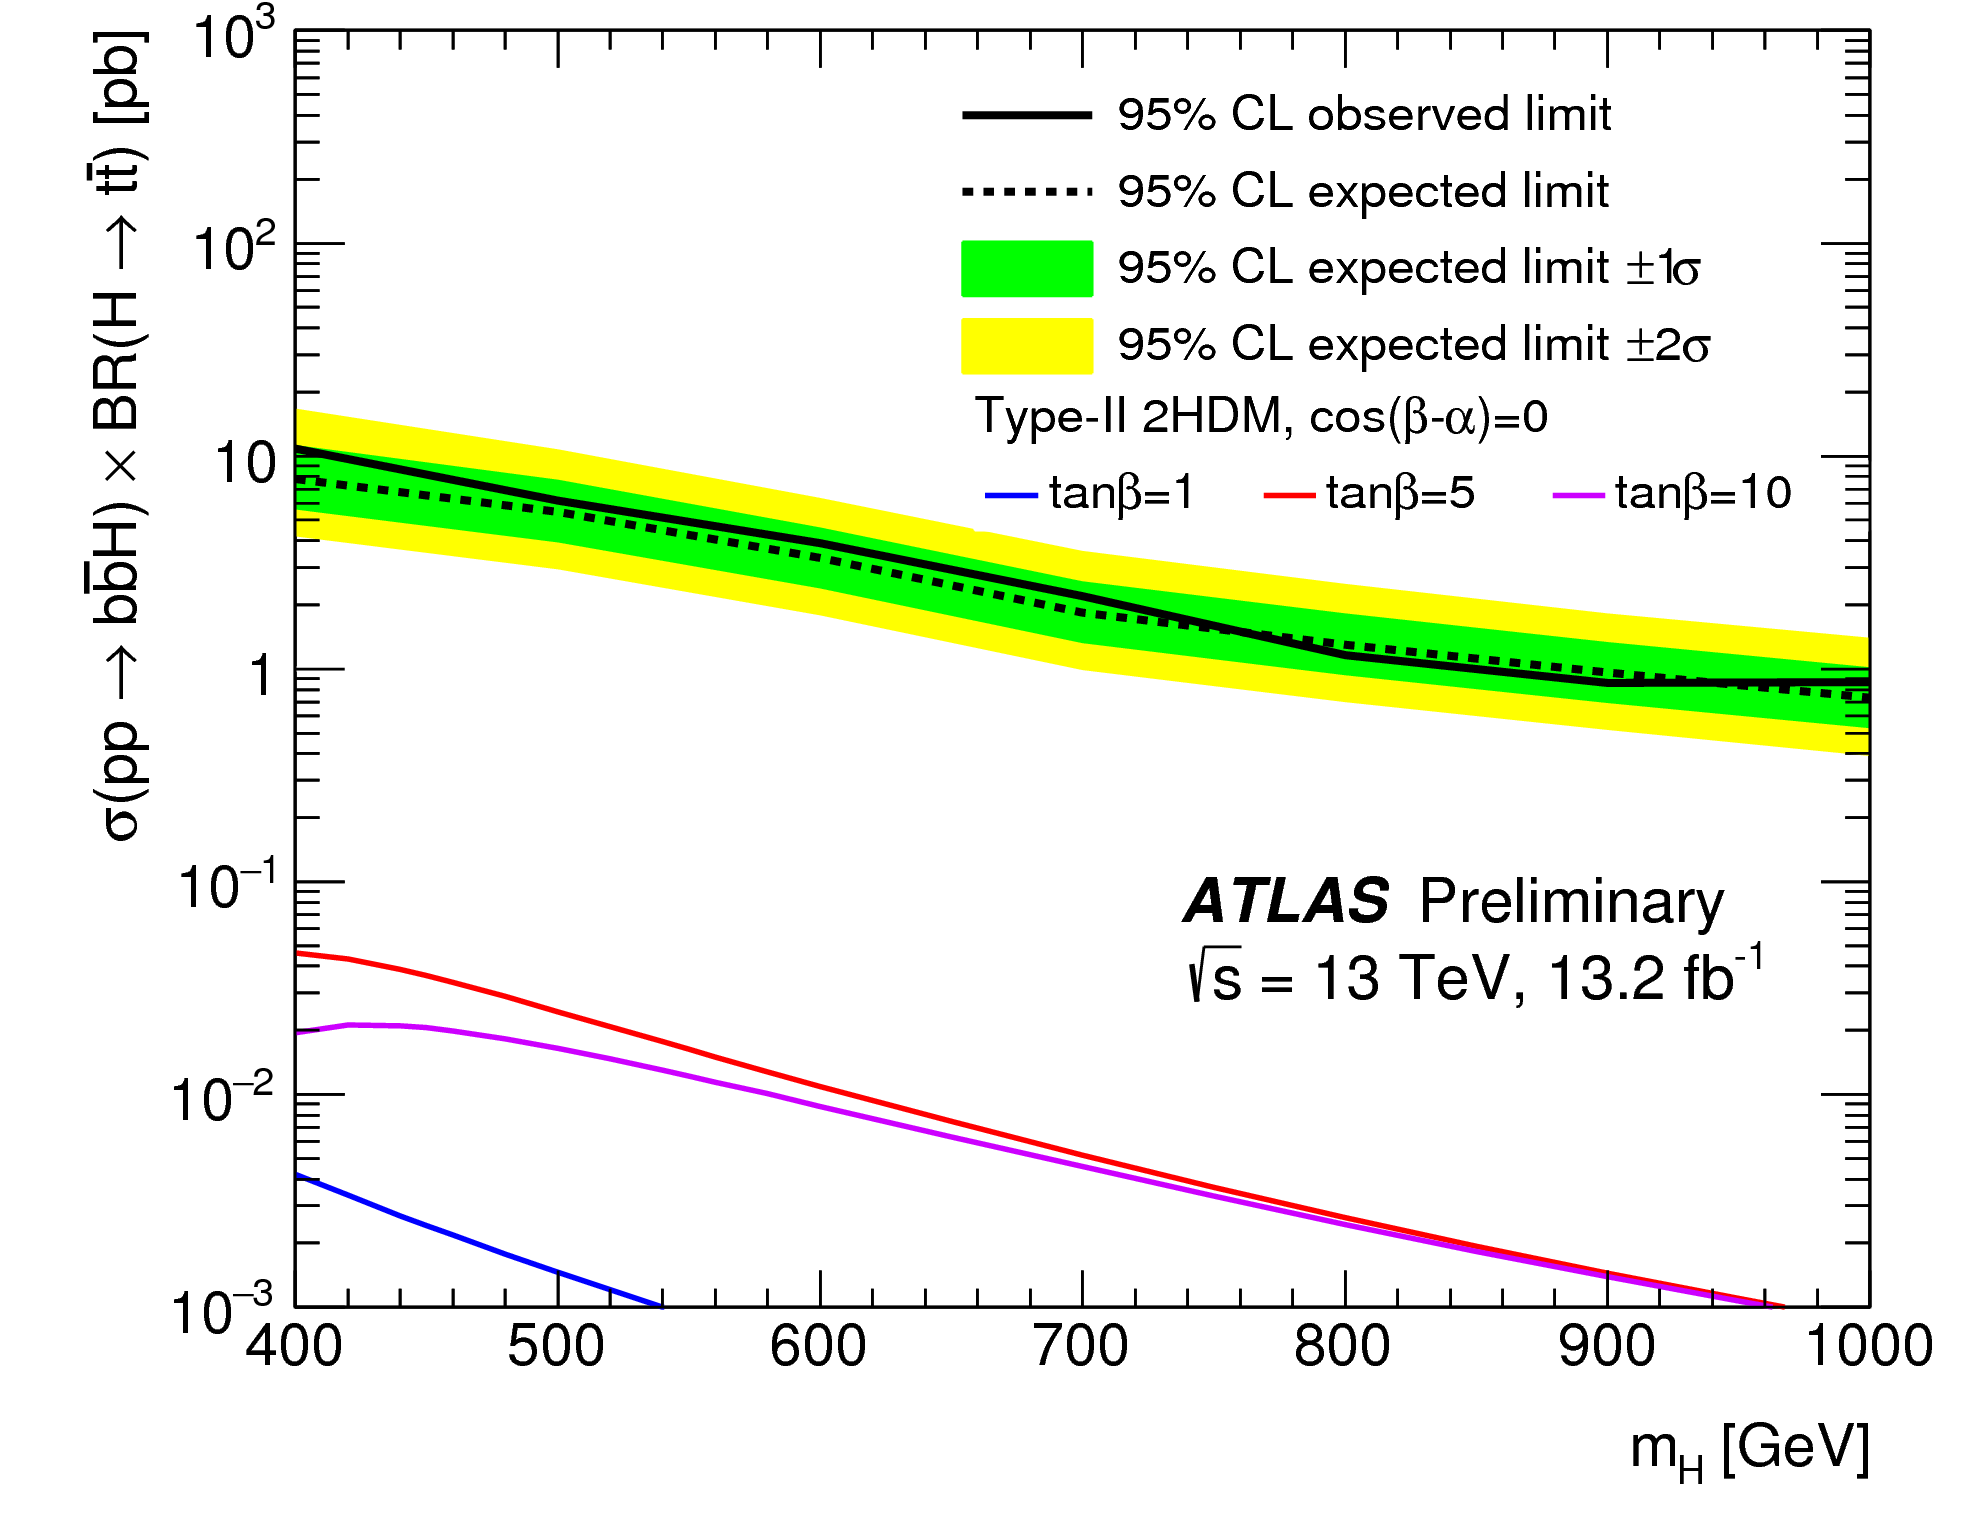
\includegraphics[width=0.9\textwidth]{figures/VLQ/fig_21b.png}
  \caption{}
  \label{}
\end{subfigure}
\captionsetup{width=0.85\textwidth} \caption{\small Observed (solid line) and expected (dashed line) 95\% CL upper limits on $\sigma(pp \to b\bar{b}H) \times {\rm BR}(H \to t\bar{t})$ 
as a function of the heavy Higgs-boson mass $m_H$, compared to the theoretical predictions assuming (a) a Type-I 2HDM, and (b) a Type-II 2HDM.
The surrounding shaded bands correspond to $\pm1$ and $\pm2$ standard deviations around the expected limit. 
The coloured thin lines show the theoretical predictions corresponding to different values of $\tan\beta$, assuming 
$\cos(\beta-\alpha)=0$.}
\label{sec:vlq:fig:hbsm1}
\end{figure}



Much better sensitivity is achieved in the $t\bar{t}H$\ search, characterised by a large multiplicity of $b$-tagged jets and mass-tagged jets.
The resulting observed and expected upper limits on $\sigma(pp \to t\bar{t}H) \times {\rm BR}(H \to t\bar{t})$ as a function of $m_H$
are shown in figure \ref{sec:vlq:fig:hbsm2}. The comparison to the predictions for a Type-I  or Type-II 
2HDM\footnote{The $ttH$ couplings have the same value in a Type-I and a Type-II 2HDM.} in the alignment limit allows the exclusion at the 95\% CL 
of $\tan\beta$ values below 0.17 (0.11) for $m_H = 400$ \gev (1 \tev). The corresponding expected lower limit is 0.23 (0.15).

\begin{figure}[h!]
\centering
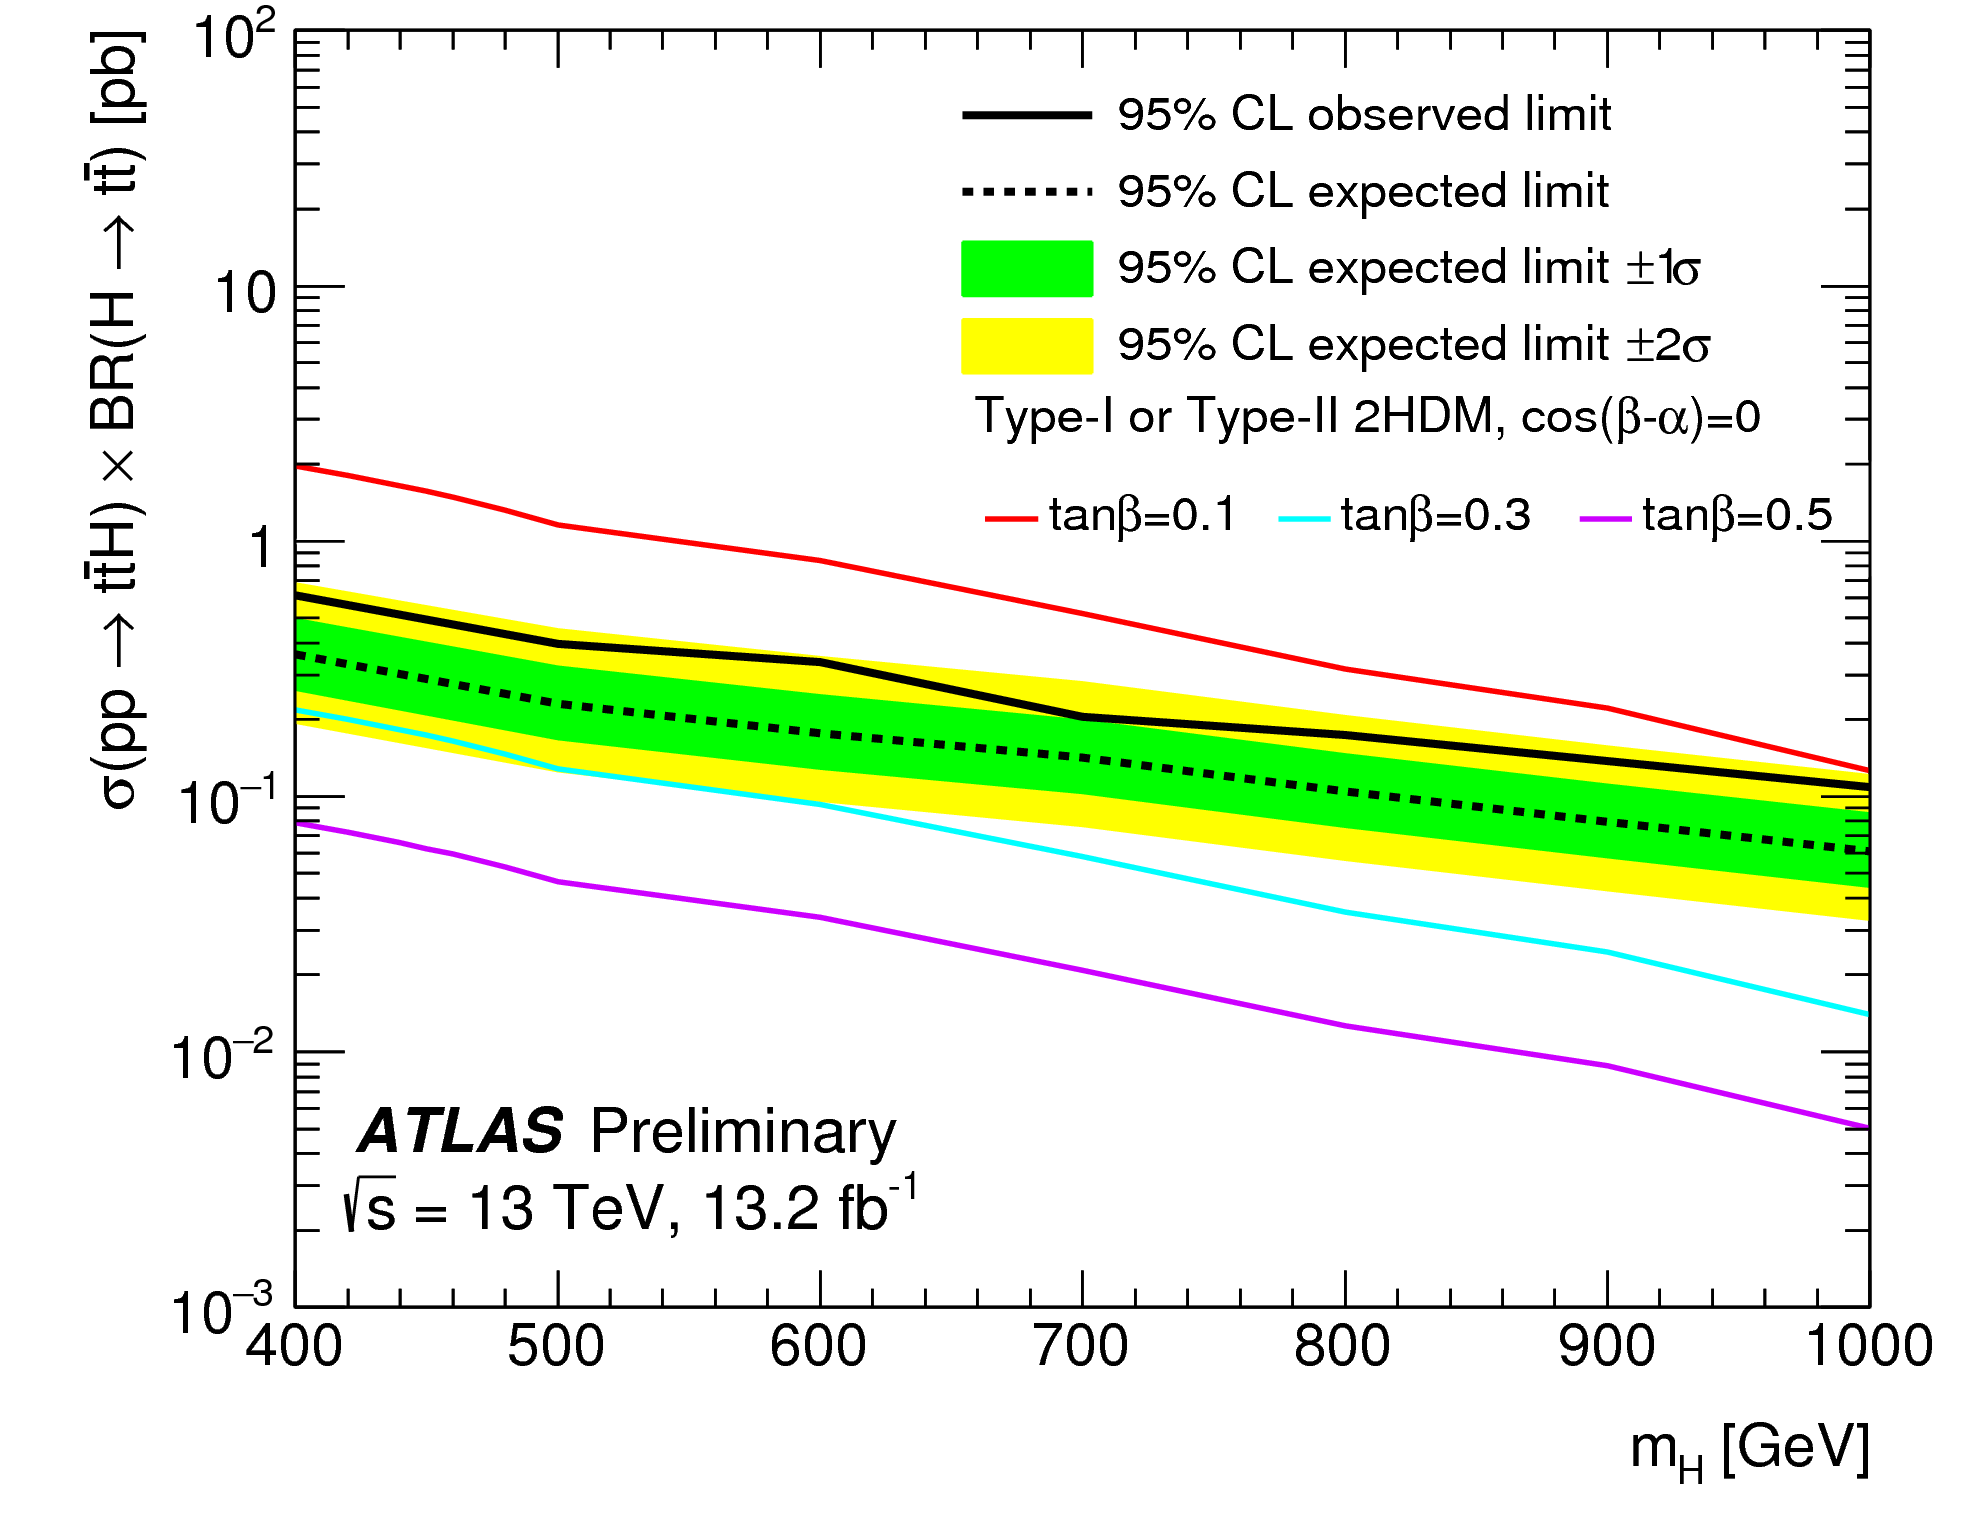
\includegraphics[width=0.5\textwidth]{figures/VLQ/fig_22.png}
\captionsetup{width=0.85\textwidth} \caption{\small Observed (solid line) and expected (dashed line) 95\% CL upper limits on $\sigma(pp \to t\bar{t}H) \times {\rm BR}(H \to t\bar{t})$ 
as a function of the heavy Higgs-boson mass $m_H$, compared to the theoretical predictions assuming a Type-I  or Type-II 2HDM.
The surrounding shaded bands correspond to $\pm1$ and $\pm2$ standard deviations around the expected limit. 
The coloured thin lines show the theoretical predictions corresponding to different values of $\tan\beta$, assuming 
$\cos(\beta-\alpha)=0$.}
\label{sec:vlq:fig:hbsm2}
\end{figure}


Finally, figure \ref{sec:vlq:fig:hbsm3} shows the observed and expected upper limits on $\sigma(pp \to \bar{t}bH^+) \times {\rm BR}(H^+ \to t\bar{b})$ 
as a function of the heavy Higgs boson mass $m_{H^+}$. The larger signal production cross section, compared to the neutral Higgs boson case,
allows to set more restrictive limits on $\tan\beta$. In this case the 95\% CL observed lower limit on $\tan\beta$ for a Type-II 2HDM is 0.65 (0.15) for 
$m_{H^{\pm}} = 200$ \gev (1 \tev). The corresponding expected lower limit is 0.55 (0.25).

\begin{figure}[h!]
\centering
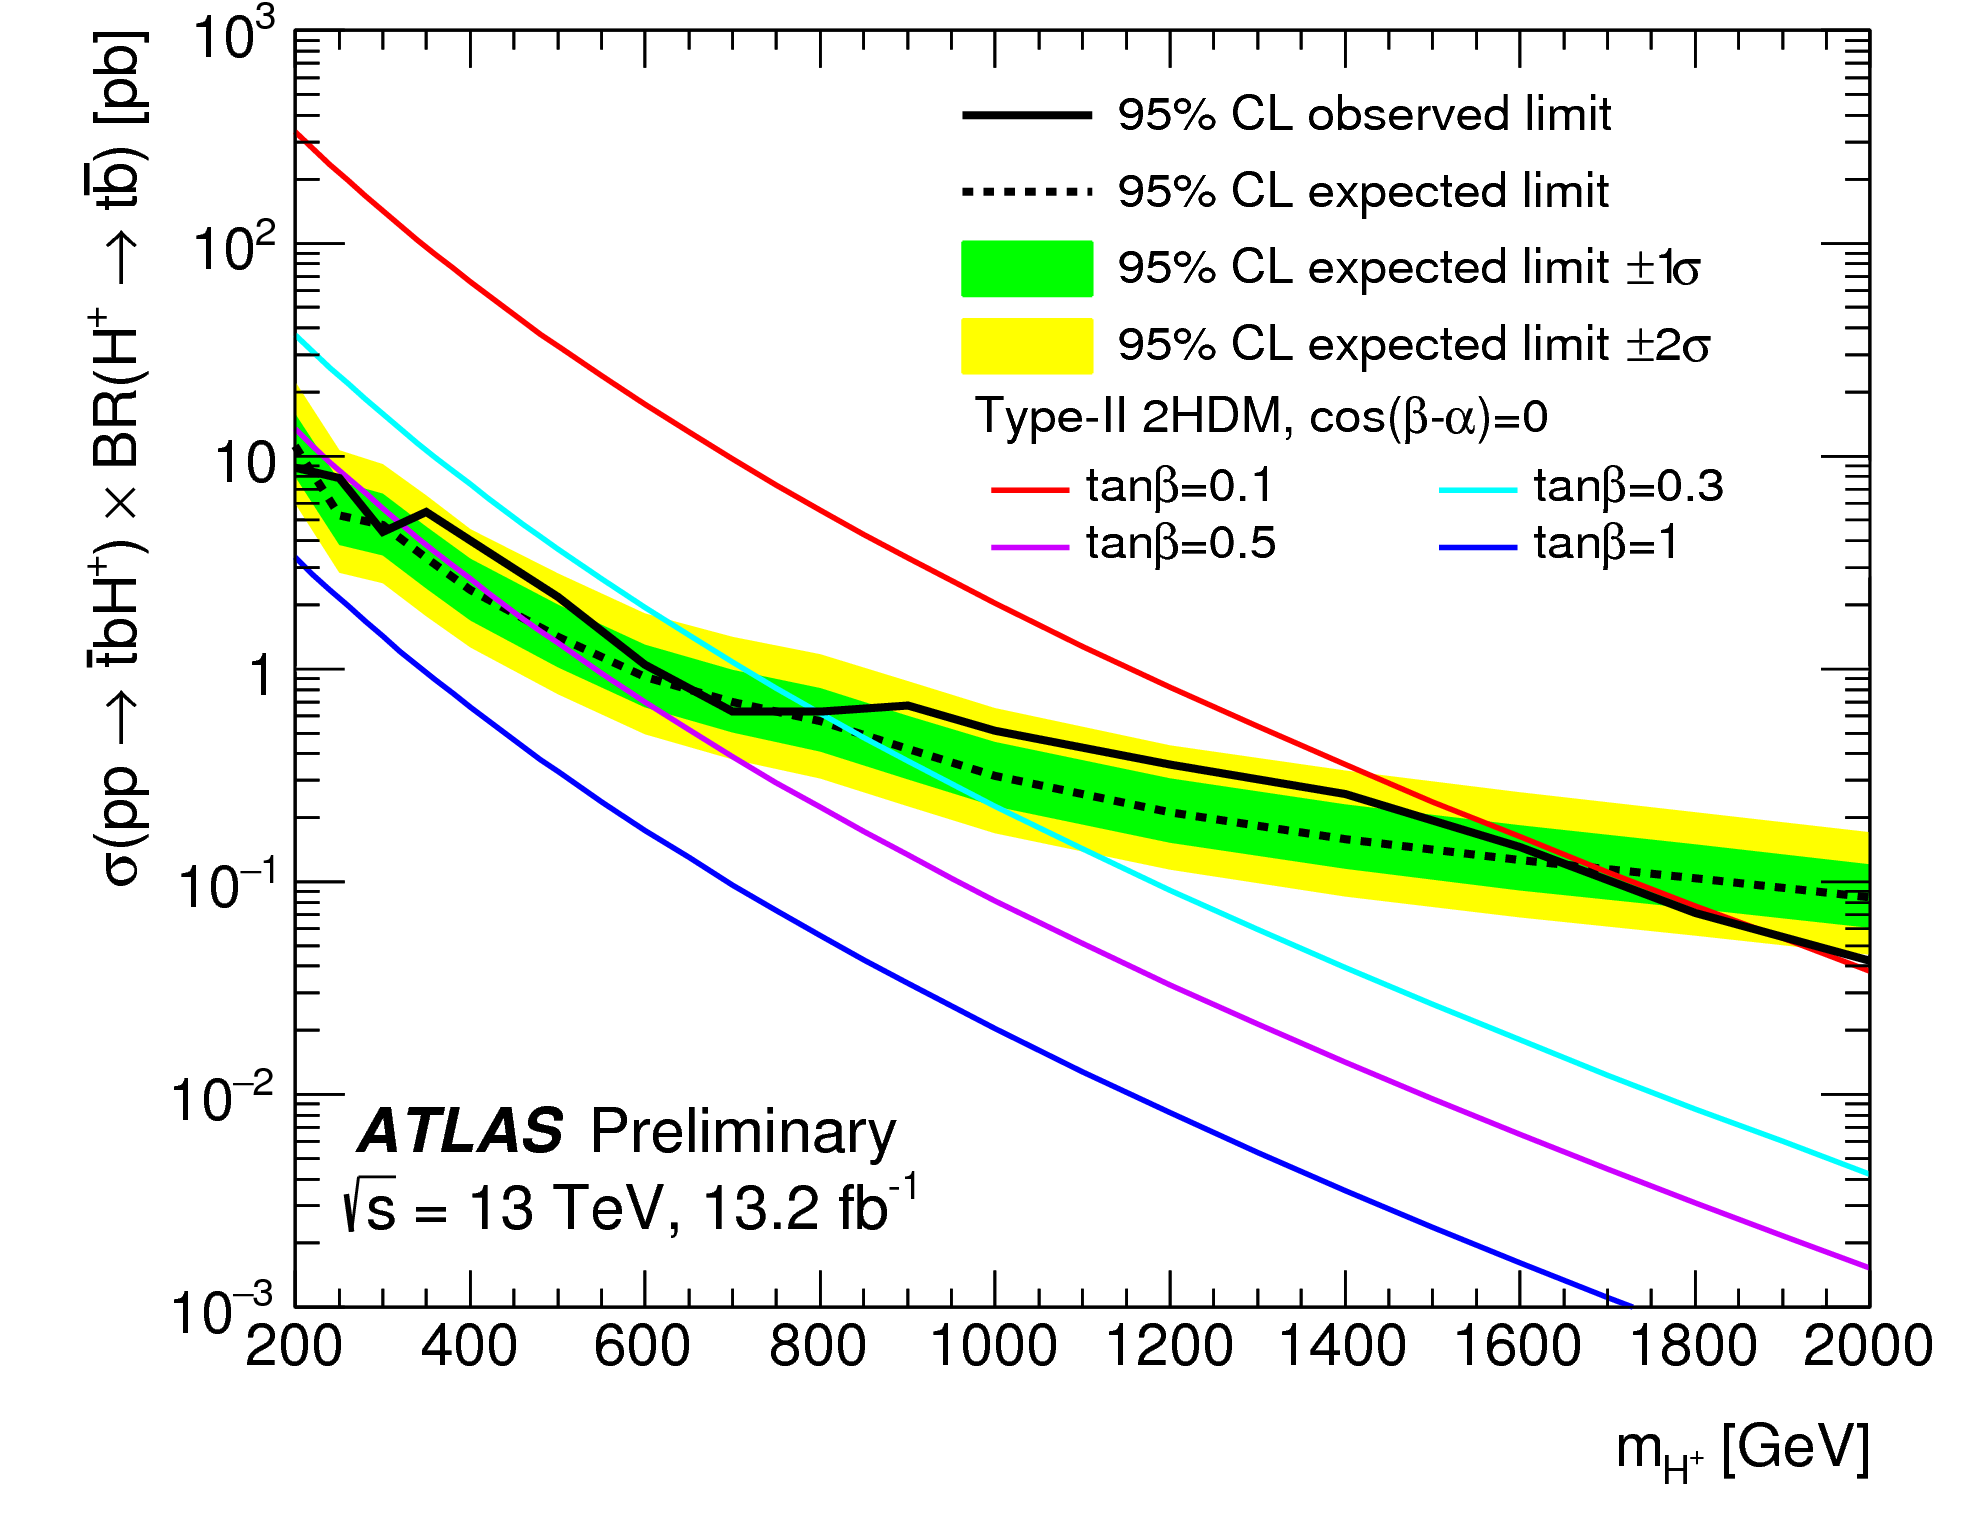
\includegraphics[width=0.5\textwidth]{figures/VLQ/fig_23.png}
\captionsetup{width=0.85\textwidth} \caption{\small Observed (solid line) and expected (dashed line) 95\% CL upper limits on $\sigma(pp \to \bar{t}bH^+) \times {\rm BR}(H^+ \to t\bar{b})$ 
as a function of the heavy Higgs-boson mass $m_{H^+}$, compared to the theoretical predictions assuming a Type-II 2HDM. 
For the values of $\tan\beta$ displayed, the predictions from a Type-I 2HDM are very close to those from a Type-II 2HDM.
The surrounding shaded bands correspond to $\pm1$ and $\pm2$ standard deviations around the expected limit. 
The coloured thin lines show the theoretical predictions corresponding to different values of $\tan\beta$, assuming 
$\cos(\beta-\alpha)=0$}
\label{sec:vlq:fig:hbsm3}
\end{figure}


The ATLAS Collaboration \cite{ATLAS-CONF-2016-089} has published a dedicated analysis targeting $tbH^{+}(\to tb)$ process with higher sensitivity compared to the analysis presented in this dissertation. It set upper limits on the cross section of 1.09--0.18 pb for $m_{H^{\pm}}=300-1000$ \gev. The interests of the analysis presented in this dissertation is that can set simultaneously limits on the three processes $b\bar{b}H$, $t\bar{t}H$, and $tbH^{+}$ and it can push the limit up to 2 $\tev$ for $tbH^{+}$ targeting boosted scenarios.  
The CMS Collaboration has not yet published results at $\sqrt{s}=13$ $\tev$ for $b\bar{b}H$, $t\bar{t}H$ and $tbH^{+}$ searches.